% \pagebreak[4]
% \hspace*{1cm}
% \pagebreak[4]
% \hspace*{1cm}
% \pagebreak[4]

\chapter{Mở đầu}
\ifpdf
    \graphicspath{{Chapter1/Chapter1Figs/PNG/}{Chapter1/Chapter1Figs/PDF/}{Chapter1/Chapter1Figs/}}
\else
    \graphicspath{{Chapter1/Chapter1Figs/EPS/}{Chapter1/Chapter1Figs/}}
\fi

\section{Giới thiệu bài toán}
Mục tiêu chính của bài toán phân lớp vật liệu là cung cấp thông tin vật liệu càng chi tiết càng tốt của một đối tượng hoặc một bề mặt trong ảnh. Hiểu một cách đơn giản, cho trước một ảnh I, máy tính cần trả lời câu hỏi "Đối tượng (hay bề mặt này) được làm từ vật liệu gì?" (chẳng hạn như gỗ, giấy, đá, kim loại, ...) (Hình \ref{fig:problem}). Ở một cấp độ cao hơn của bài toán, máy tính cần cho biết chính xác loại vật liệu của từng pixel trên ảnh (Hình \ref{fig:seg}). Trong luận văn này, nhóm giải quyết câu hỏi thứ nhất.

\begin{figure}[h!]
	\centering
	\captionsetup{width=0.9\textwidth}
	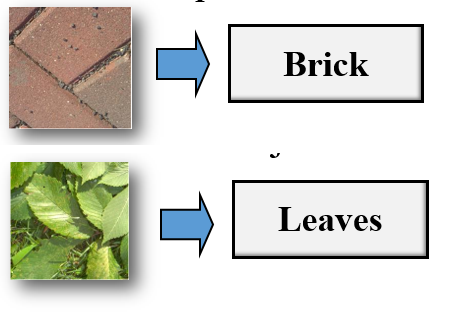
\includegraphics[width=0.5\textwidth]{problem.png}
	\caption{Phân lớp vật liệu cho biết bề mặt trong ảnh thuộc vật liệu nào}
    \label{fig:problem}
\end{figure}

\begin{figure}[h!]
	\centering
	\captionsetup{width=0.9\textwidth}
	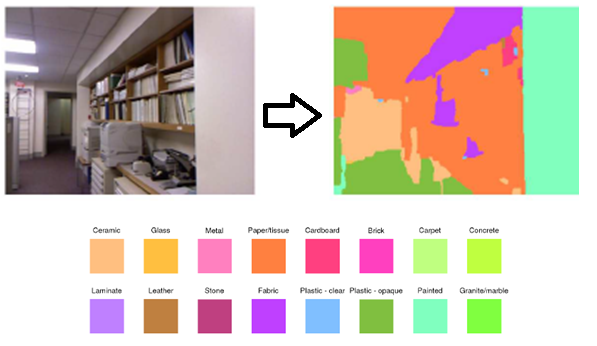
\includegraphics[width=0.8\textwidth]{segmentation.png}
	\caption{Phân lớp vật liệu cho biết chính xác vật liệu của từng pixel trong ảnh}
    \label{fig:seg}
\end{figure}

\pagebreak

\section{Tại sao cần phân lớp vật liệu?}
\paragraph*{}
Vật liệu của một bề mặt hay đối tượng nào đó là một thông tin rất giá trị để máy tính của thể hiểu được các thuộc tính của nó và từ đó có thể đưa ra các quyết định liên quan cũng như tương tác với chúng. Hình \ref{fig:bottles} và \ref{fig:car} là hai ví dụ đơn giản cho thấy máy tính có thể làm được rất nhiều việc khi có thể biết được thông tin về vật liệu. Trong hình \ref{fig:bottles}, với thông tin về vật liệu của các chai nước này này, đơn giản nhất máy tính có thể sắp xếp chúng theo cân nặng, ngoài ra còn có thể quyết định chai nào có thể được dùng để đựng nước nóng chai nào không thể hay thậm chí chai nào có thể sử dụng để gây sát thương cho người khác (chai thủy tinh

\begin{figure}[h!]
	\centering
	\captionsetup{width=0.9\textwidth}
	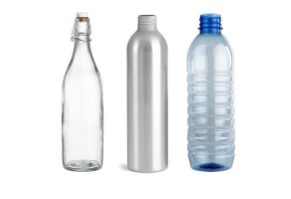
\includegraphics[width=0.8\textwidth]{bottles.png}
	\caption{Ba chai đựng nước với hình dáng tương tự nhau được làm từ những vật liệu khác nhau - quyết định những tính chất vật lý khác nhau}
    \label{fig:bottles}
\end{figure}

\begin{figure}[h!]
	\centering
	\captionsetup{width=0.9\textwidth}
	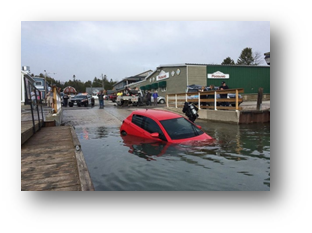
\includegraphics[width=0.8\textwidth]{car.png}
	\caption{Xe tự lái: "Xin lỗi, tôi không biết đó là nước :("}
    \label{fig:car}
\end{figure}

\paragraph*{}
Ngoài ra, vật liệu còn là một chìa khóa quan trọng để cải tiến bài toán "Scene understanding" trong Thị Giác Máy Tính \cite{corbettreal} và còn được ứng dụng trong nhiều lĩnh vực khác nhau trong đời sống như các hệ thống xe tự lái (Advanced Driver-Assistance Systems) \cite{r1}, Robotic Manipulation \cite{spong2006robot} hay Robotic Navigation \cite{kim2013robot}. 

\section{Các thách thức của bài toán}
Nhiều thách thức khác nhau kết hợp làm bài toán phân lớp vật liệu rất khó giải quyết triệt để. Sự đa dạng về hình dáng, kích thước và texture là một trong số đó, có rất nhiều đối tượng có hình dáng khác nhau nhưng lại cùng loại vật liệu, ngược lại có những đối tượng trông có vẽ rất giống nhau nhưng lại làm từ những vật liệu khác nhau. Ngoài ra, điều kiện chiếu sáng khác nhau cũng khiến việc phân biệt giữa các vật liệu trở nên rất khó khăn (đặc biết đối với việc chỉ dùng một ảnh màu để phân biệt). Bên cạnh đó, sự chồng lắp giữa các đối tượng với nhau, giữa đối tượng với background cũng là một thách thức không nhỏ. Hình \ref{ex1} và \ref{ex2} là hai ví dụ cho thấy bài toán này thật sự rất thách thức.

\begin{figure}[h!]
	\centering
	\captionsetup{width=0.9\textwidth}
	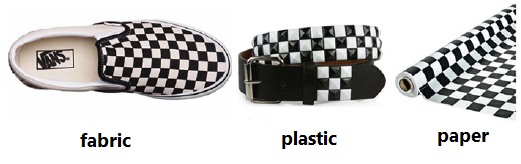
\includegraphics[width=0.8\textwidth]{ex1.png}
	\caption{Những đối tượng với chất liệu khác nhau nhưng bề mặt lại có texture giống nhau (đều là sọc ca-rô)}
    \label{fig:ex1}
\end{figure}

\begin{figure}[h!]
	\centering
	\captionsetup{width=0.9\textwidth}
	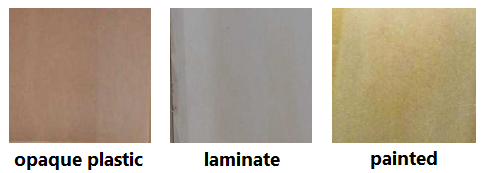
\includegraphics[width=0.8\textwidth]{ex2.png}
	\caption{Một ví dụ từ tập dữ liệu Open-Surface cho thấy bài toán này thách thức như thế nào}
    \label{fig:ex2}
\end{figure}

